\documentclass[10pt,paper=letter]{scrartcl}
\usepackage[alttitle]{cjquines}

\begin{document}

\title{VCSMS PRIME}
\subtitle{Program for Inducing Mathematical Excellence}
\author{Session 4: Counting and Probability}
\date{September 22, 2017}

\maketitle
\setlength{\unitlength}{1in}
\begin{picture}(0,0)
  \put(5.5,0.5){\hbox{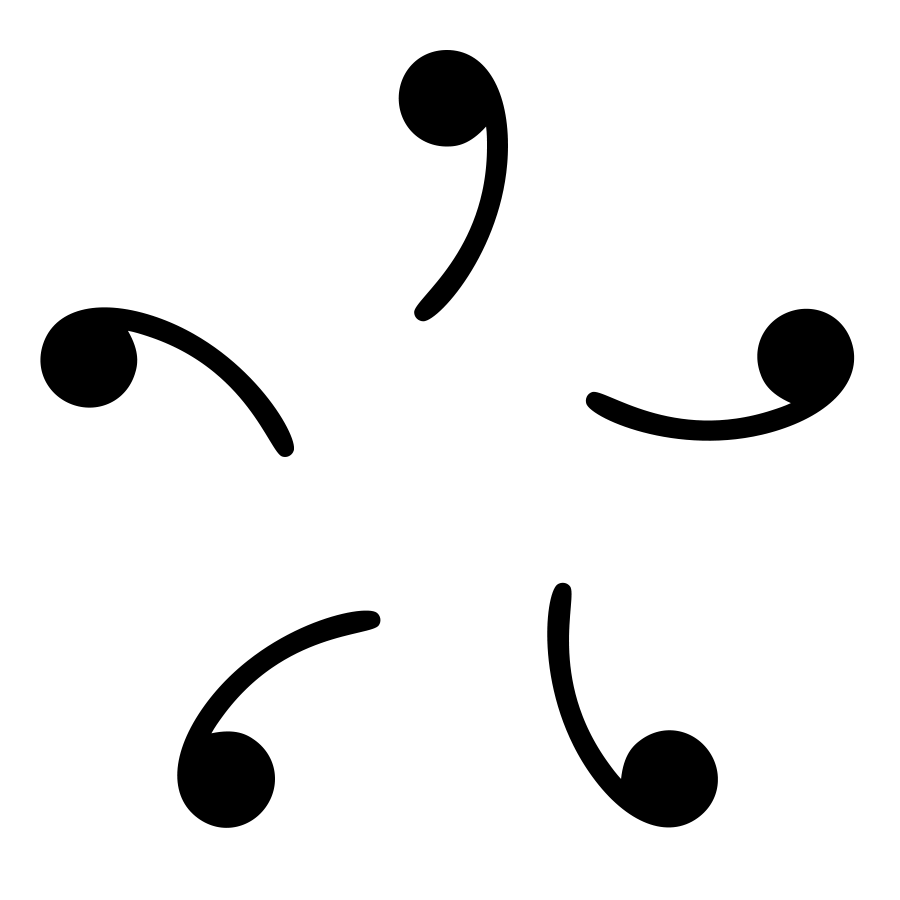
\includegraphics[width=0.9in]{logo.png}}}
\end{picture}
\vspace{-3.5em}

\subsubsection*{Lecture problems}

\begin{enumerate}
  \item (QI7) Issa has an urn containing only red and blue marbles. She selects a number of marbles from the urn at random and without replacement. She needs to draw at least $N$ marbles in order to be sure that she has at least two red marbles. In contrast, she needs three times as much in order to be sure that she has at least two blue marbles. How many marbles are there in the urn?
  \item I flip a coin. If it comes up heads I roll two dice and if it comes up tails I roll three dice. Given that the sum of the dice is $4$, what is the probability I flipped heads?
  \item At a nursery, $2006$ babies sit in a circle. Suddenly, each baby randomly pokes either the baby to its left or its right. What is the expected number of unpoked babies?
  \item (QII7) Louie plays a game where he throws a circular coin with radius $1$ unit, which falls flat entirely inside a square board having side $10$ units. He wins the game if the coin touches the boundary or the interior of a circle of radius $2$ units drawn at the center of the board. What is the probability that Louie wins the game?
  \item (QII8) Guido and David each randomly choose an integer from $1$ to $100$. What is the probability that neither is the square of the other?
  \item (AI7) A small class of nine boys are to change their seating arrangement by drawing their new seat numbers from a box. After the seat change, what is the probability that there is only one pair of boys who have switched seats with each other and only three boys who have unchanged seats?
  \item (AI18) A railway passes through four towns $A, B, C,$ and $D$. The railway forms a complete loop, as shown on the right, and trains go in both directions. Suppose that a trip between two adjacent towns costs one ticket. Using exactly eight tickets, how many distinct ways are there of traveling from town $A$ and ending at town $A$? (\emph{Note that passing through $A$ somewhere in the middle of the trip is allowed.})
\end{enumerate}

\subsubsection*{Shooting pigeons}

\begin{itemize}
  \item Existence: is there or is there not? Versus enumerative: how many?
  \item Pigeonhole principle: if you have $n$ pigeons and $n+1$ holes then at least one pigeon will have more than one hole. (Or if you put $n+1$ pigeons into $n$ holes, but that's more boring.)
  \item Drawer principle: if you have $a$ red socks and $b$ non-red socks in a drawer, you have to pick $b+1$ socks to assure you get at least one red sock. 
  \item Problem 1: direct application of drawer principle.
  \item Think of ``worst-case'' scenario and go from there. Related:
  \begin{itemize}
    \item How many socks to pick to ensure at least one of each color?
    \item How many integers do you have to pick to ensure some two of these integers have a difference that is divisible by four?
    \item How many points do you have to pick in a square of side $2$ to ensure two of them are within distance $\sqrt{2}$ of each other?
  \end{itemize}
\end{itemize}

\newpage

\subsubsection*{Probabilities}

\begin{itemize}
  \item Problem 2: Conditional probability: $P(A|B) = P(AB)/P(B)$.
  \item Expected value is its ``average''. Expected value of a dice roll is $3.5$. Expected number of heads in three coin tosses is $1.5$. It is linear: if you roll $100$ dice you expect an average of $350$. But this is true even if it is not independent.
  \item Problem 3: Just consider one baby and multiply by 2006.
  \item Geometric probability is dividing the areas. Sometimes it comes up in unexpected ways, like when choosing real numbers (dividing lengths). Sometimes it is helpful to graph and find the areas.
  \item Problem 4: Draw a picture! Key idea is to consider center of coin: where can it fall so that Louie wins?
\end{itemize}

\subsubsection*{Counting the wrong thing}

\begin{itemize}
  \item Sometimes it is easier to count the opposite and subtract: \emph{complementary counting}.
  \item How many ways to sit six people in a row so two particular people don't sit next to each other?
  \item I choose four letters at random, what's the probability I chose the same letter twice?
  \item Problem 5: Instead of ``neither is the square of the other'', what about the probability one of them is the square of the other?
\end{itemize}

\subsubsection*{Brute force}

% ad hoc: 2 3 5 10
% brute force

\begin{itemize}
  \item Count manually. Five cases out of twelvefold way.
  \item How many ways to rearrange four letters so no letter is in its own place and no two letters have swapped?
  \item Problem 6: There are $\binom{9}{2}$ ways to pick two boys who switch, and $\binom{7}{3}$, out of the remaining $7$ boys, to pick three unchanged. Then there are $6$ ways for the remaining four boys. 
  \item Divide into cases: how many odd numbers with middle digit $5$, no digit repeated, between $20000$ and $69999$?
\end{itemize}

\subsubsection*{``Carefully''}

\begin{itemize}
  \item How do you solve hard combinatorics problems?
  \item Problem 7: How can represent a trip? We can do it using towns, but that would be too hard. It is easier to represent with ``left'' and ``right''. Divide into cases and use the identity from yesterday.
  \item Often problems don't involve only one technique, but several. Make sure to remember all the principles, be creative, and try many different ways until you find one that works.
\end{itemize}

\end{document}
